\documentclass[11pt,a4paper]{article}
\usepackage[margin=2.5cm]{geometry}
\usepackage{booktabs}
\usepackage{listings}
\usepackage{xcolor}
\usepackage{graphicx}
\usepackage{float}

\lstset{
  basicstyle=\ttfamily\small,
  frame=single,
  backgroundcolor=\color{gray!8},
  breaklines=true
}

\title{Labwork 5: Gaussian Blur Convolution}
\author{Yanis Denizot -- 2640051}
\date{\today}

\begin{document}
\maketitle

\section{Implementation}
I used the 2D kernel of labwork 4 and changed the computation to a $7 \times 7$ Gaussian blur.
For each pixel and each color channel, the new value is the weighted average of the
$7 \times 7$ neighbors, with the weights of the Gaussian filter from the course (sum = 1003).
On the borders, the neighbors outside the image are skipped, and I divide by the sum of the
weights that were really used.

Without shared memory, the filter is read from global memory:
\begin{lstlisting}[language=Python]
@cuda.jit
def blur(src, dst, filt):
    x = cuda.threadIdx.x + cuda.blockIdx.x * cuda.blockDim.x
    y = cuda.threadIdx.y + cuda.blockIdx.y * cuda.blockDim.y
    h = src.shape[0]
    w = src.shape[1]
    if y < h and x < w:
        for c in range(3):
            s = 0.0
            wsum = 0.0
            for i in range(7):
                for j in range(7):
                    ny = y + i - 3
                    nx = x + j - 3
                    if ny >= 0 and ny < h and nx >= 0 and nx < w:
                        s += src[ny, nx, c] * filt[i, j]
                        wsum += filt[i, j]
            dst[y, x, c] = np.uint8(s / wsum)
\end{lstlisting}

With shared memory, the first $7 \times 7$ threads of each block copy the filter into shared
memory, then \texttt{cuda.syncthreads()} makes all the threads wait until the copy is
finished. The rest of the kernel is the same, but it reads \texttt{sfilt} instead of
\texttt{filt}. The \texttt{syncthreads()} must be before the border check, otherwise the
threads outside the image never reach it.
\begin{lstlisting}[language=Python]
    sfilt = cuda.shared.array((7, 7), np.float32)
    tx = cuda.threadIdx.x
    ty = cuda.threadIdx.y
    if tx < 7 and ty < 7:
        sfilt[ty, tx] = filt[ty, tx]
    cuda.syncthreads()
\end{lstlisting}

The image is $1200 \times 800$ pixels. The CPU version (Python loops) takes 233 s. Both GPU
versions give exactly the same image as the CPU (maximum difference = 0).

\begin{figure}[H]
\centering
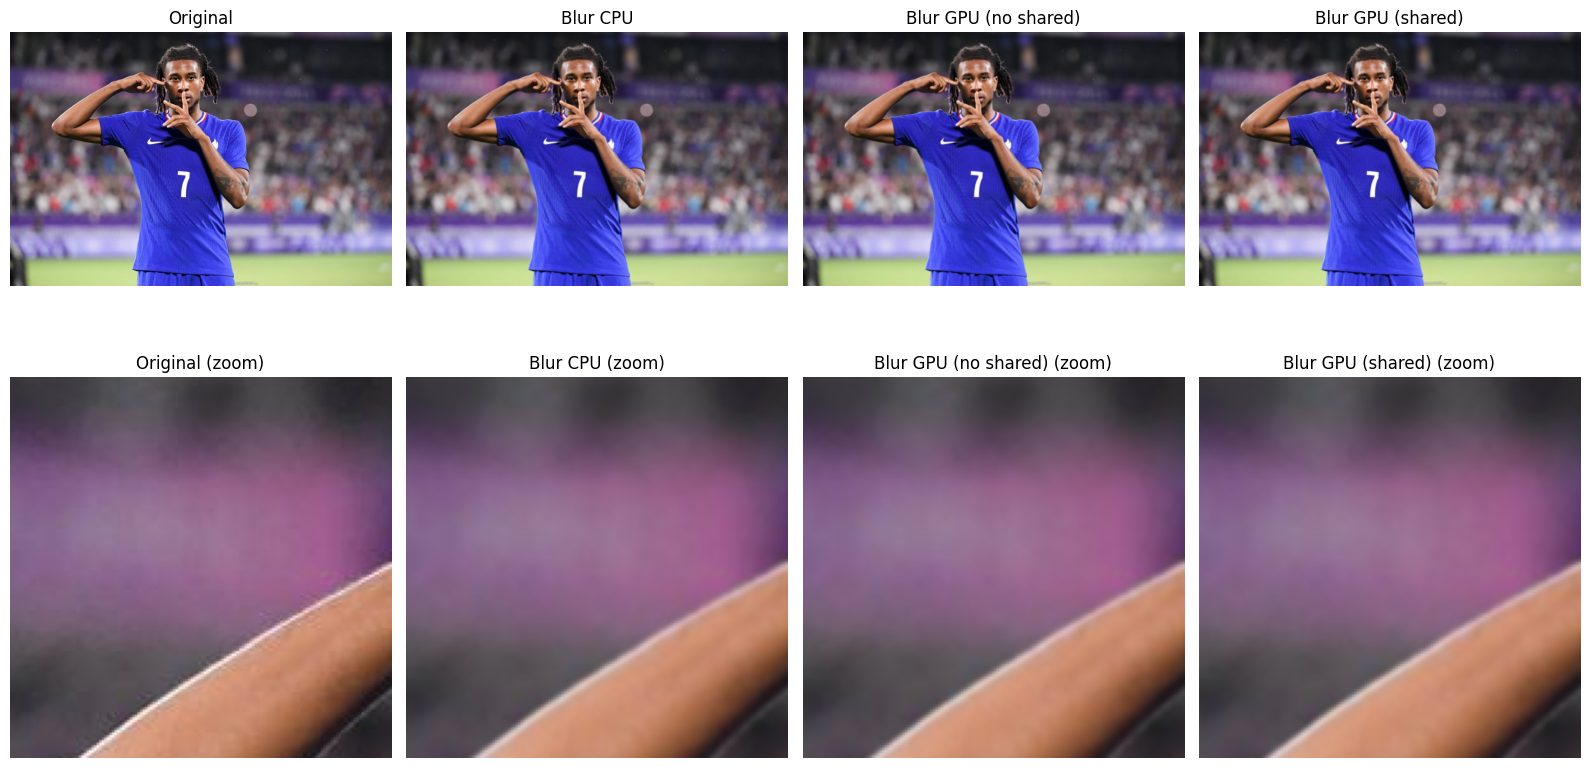
\includegraphics[width=\textwidth]{comparison.png}
\caption{Original image and blurred results (top), and a zoom (bottom)}
\end{figure}

\section{Results}
For each block size, the GPU time is the average of 100 launches.

\begin{table}[H]
\centering
\begin{tabular}{lrrrr}
\toprule
Block & No shared (ms) & Shared (ms) & No shared speedup & Shared speedup \\
\midrule
$8 \times 8$   & 6.82 & 5.30 & 34194 & 44043 \\
$16 \times 8$  & 5.30 & 5.31 & 44001 & 43974 \\
$16 \times 16$ & 5.29 & 5.29 & 44083 & 44071 \\
$32 \times 16$ & 5.40 & 5.40 & 43192 & 43171 \\
$32 \times 32$ & 5.44 & 5.44 & 42861 & 42849 \\
\bottomrule
\end{tabular}
\end{table}

\begin{figure}[H]
\centering
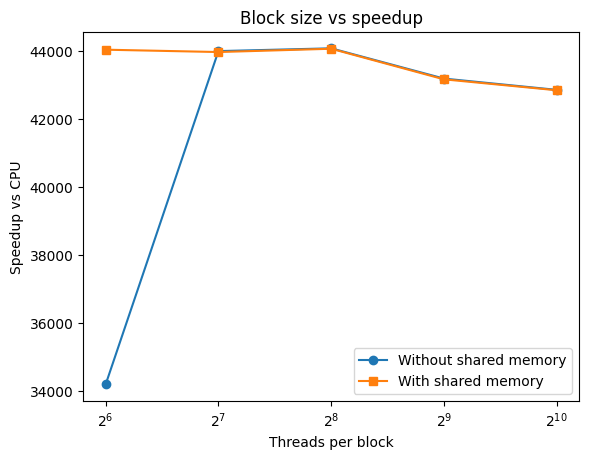
\includegraphics[width=0.65\textwidth]{blocksize_vs_speedup.png}
\end{figure}

The speedup is very high (around 44000) because the blur needs $7 \times 7 \times 3 = 147$
operations per pixel, which is very slow in Python on the CPU.

Shared memory only helps with $8 \times 8$ blocks (22\% faster). For the other block sizes,
the two versions have the same time. I think this is because all the threads of a warp read
the same value of the filter at the same time, and the filter is very small (49 values), so
it stays in the cache and is already fast without shared memory. With $8 \times 8$ blocks, a
warp covers 4 different rows of the image, so the image reads use more of the cache and the
filter is probably removed from it more often. In shared memory, the filter always stays
available. I checked this point twice and got the same result. As in the previous labworks,
the biggest blocks ($32 \times 32$) are a bit slower.

\end{document}
